% Schematic representation of mach zender interferometer
% Modified from a version created by Henrik Kröger, https://github.com/derhedwig/fiberoptics/blob/master/auswertung.tex
% Author: Orlando Torres (2016)

\documentclass{standalone}
\usepackage{amsmath} % Required for \varPsi below
\usepackage{tikz,pgfplots}
\usetikzlibrary{calc}
\usetikzlibrary{patterns}

\begin{document}
  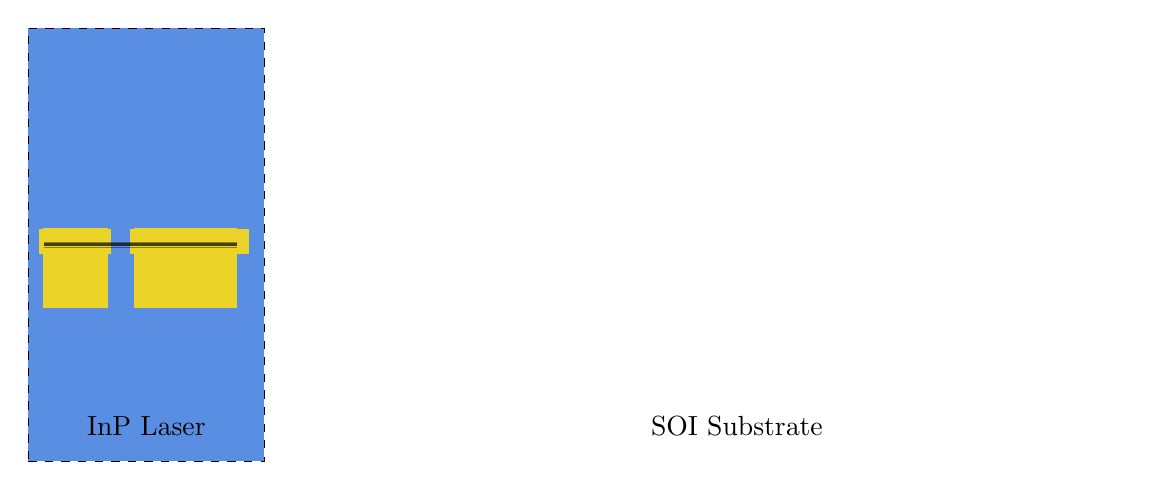
\begin{tikzpicture}
   	%define colors
    \definecolor{bbblue}{rgb}{0.964, 0.866, 0.474}
    \definecolor{rrred}{rgb}{0.952, 0.815, 0.105}
    \definecolor{yyyellow}{rgb}{0.925, 0.827, 0.152}    
    %0.933, 0.756, 0.227
    \definecolor{lblue}{rgb}{0.352, 0.556, 0.886}
    \definecolor{sblue}{rgb}{0.607, 0.733, 0.929}
	\definecolor{lyel}{rgb}{0.925, 0.827, 0.152}
    
    %define coordinates for PWB (center)
    \coordinate (PWBin) at (-63.0mm, 0);
    %define coordinates for modulator (upper side)
    \coordinate (in) at (-50.0mm, 0);
    \coordinate (in0) at (-35mm, 0);
    \coordinate (in0a) at (-35mm, 1.2mm);
    \coordinate (in0b) at (-25mm, 1.2mm);
    \coordinate (in1) at (-20mm, 9mm);
    \coordinate (out1) at (20mm, 9mm);
    \coordinate (out0b) at (25mm, 1.2mm);
    \coordinate (out0a) at (35mm, 1.2mm);
    \coordinate (out0) at (35mm, 0);
    \coordinate (out) at (50.0mm, 0);
    %define coordinates for modulator (lower side)
    \coordinate (in1a) at (-35mm, -1.2mm);
    \coordinate (in1b) at (-25mm, -1.2mm);
    \coordinate (in2) at (-20mm, -9mm);
    \coordinate (out2) at (20mm, -9mm);
    \coordinate (out1a) at (35mm, -1.2mm);
    \coordinate (out1b) at (25mm, -1.2mm);
    
    %Location of the Signal/Ground/Signal indicators
    \coordinate (phmod) at (-20mm, 4mm);
    \coordinate (gen) at (0mm, 0);
    %\coordinate (gen1) at ($ (gen) + (0, 15mm) $);
    %\coordinate (gen2) at ($ (gen) + (0, -15mm) $);
    \coordinate (ter) at (12mm, 0);
     %Location of the arrow polarization indicators
    \coordinate (arr0) at (-10mm,-13mm);
    \coordinate (arr1) at (-10mm,13mm);
    \coordinate (arrRF0p) at (7.5mm,-15mm);
    \coordinate (arrRF1p) at (7.5mm,-4mm);
    \coordinate (arrRF0n) at (7.5mm,15mm);
    \coordinate (arrRF1n) at (7.5mm,4mm);
    
    % Substrate, modulators, Waveguides, MMI and converters %
    
    \node [shape=rectangle, minimum width=30mm, minimum height=55mm, color=black, fill=lblue, draw,dashed]
    (lasersubs) at (-75mm,0) {}; 
    
    %\node [shape=rectangle, minimum width=105mm, minimum height=55mm, color=black, draw,fill=sblue,dashed]
    %(substrate) at (0,0) {};
    %\node [shape=rectangle, minimum width=37.1mm, minimum height=15.5mm, color=yyyellow,fill=yyyellow,  draw] (emid) {};
    %\node [shape=rectangle, minimum width=37.1mm, minimum height=8mm, color=yyyellow,above=10.2mm, fill=yyyellow, draw](etop) {}; 
    %\node [shape=rectangle, minimum width=37.1mm, minimum height=8mm, color=yyyellow,below=10.2mm, fill=yyyellow, draw] (ebot) {};
%	\draw  [line width=2.50mm, color=gray] (in1) -- (out1);
%	\draw  [line width=2.50mm, color=gray] (in2) -- (out2);
	
	%Laser
    \node [shape=rectangle, minimum width=8mm, minimum height=10mm, color=lyel, fill=lyel, draw] (lmirr1) at (-84mm,-3mm) {};	
	\node [shape=rectangle, minimum width=13mm, minimum height=10mm, color=lyel, fill=lyel, draw] (lmirr2) at (-70mm,-3mm) {};
	
	\node [shape=rectangle, minimum width=9mm, minimum height=3mm, color=lyel, fill=lyel, draw] (lgn1) at (-84mm,0.4mm) {};
	\node [shape=rectangle, minimum width=15mm, minimum height=3mm, color=lyel, fill=lyel, draw] (lgn2) at (-69.5mm,0.4mm) {};
	\draw  [line width=0.40mm, color=black,opacity=0.7] (-88mm,0mm) -- (-63.5mm,0mm);
	\draw  [line width=0.10mm, color=black,opacity=0.4] (-88mm,0.35mm) -- (-63.5mm,0.35mm);
	\draw  [line width=0.10mm, color=black,opacity=0.4] (-88mm,-0.35mm) -- (-63.5mm,-0.35mm);

    % Optical path %
%    \draw  [line width=1.00mm, color=black] (in) -- (in0) -- (in0a) -- (in0b) -- (in1) -- (out1) -- (out0b) --  (out0a) --
%    (out0) -- (out);
%    \draw  [line width=0.5mm, color=white] (in1) -- (out1);
%    \draw  [line width=1.00mm, color=black] (in) -- (in0) -- (in1a) -- (in1b) -- (in2) -- (out2) -- (out1b) -- (out1a) --
%    (out0) -- (out);
    %PWB
    %\draw [line width=1.20mm,red] plot [smooth, tension=1] coordinates {($ (PWBin) + (-2mm, 0mm) $)  ($ (PWBin) + (1mm, 1mm) $) ($ (PWBin) + (5mm, 5mm) $) ($ (in) + (-3mm, 1mm) $) ($ (in) + (2mm, 0mm) $)};
    
    %\draw [fill=orange] (lasersubs) rectangle (0.2,0.2);
    %Slot waveguide
	\draw  [line width=0.5mm, color=white] (in2) -- (out2);
	%Poling and local RF field
    %\draw [->, to path={-| (\tikztotarget)},line width=0.50mm, color=blue, dashed]  (arr0) -- (arr1);
    %\draw [->, to path={-| (\tikztotarget)},line width=0.70mm, color=red, dotted] (arrRF1p) -- (arrRF0p);
   % \draw [->, to path={-| (\tikztotarget)},line width=0.70mm, color=red, dotted] (arrRF1n) -- (arrRF0n);
	
%	\node [shape=rectangle, minimum width=3mm, minimum height=2.5mm,fill=rrred, draw]
%    (substrate) at (20mm,-9mm) {};
%	\node [shape=rectangle, minimum width=7mm, minimum height=5mm,color=bbblue,fill=bbblue, draw]
%    (substrate) at (-35mm,0) {};
%    \node [shape=rectangle, minimum width=7mm, minimum height=5mm,color=bbblue,fill=bbblue, draw]
%    (substrate) at (35mm,0) {};
%    \node [shape=rectangle, minimum width=3mm, minimum height=2.5mm,color=gray,fill=rrred, draw]
%    (substrate) at (-20mm,9mm) {};
%    \node [shape=rectangle, minimum width=3mm, minimum height=2.5mm,color=gray,fill=rrred, draw]
%    (substrate) at (20mm,9mm) {};
%    \node [shape=rectangle, minimum width=3mm, minimum height=2.5mm,color=gray,fill=rrred, draw]
%    (substrate) at (-20mm,-9mm) {};
%    \node [shape=rectangle, minimum width=3mm, minimum height=2.5mm,color=gray,fill=rrred, draw]
%    (substrate) at (20mm,-9mm) {};
	
    % Connections %
    %\draw (gen) node [shape=circle, color=black, fill=white, inner sep=1, draw]
    %(gen_node) {S};
    %\draw (gen) node [shape=circle, color=black, fill=white, inner sep=0.6, draw]
    %(gen1_node) at +(0, 14mm) {G};
    %\draw (gen) node [shape=circle, color=black, fill=white, inner sep=0.6, draw]
    %(gen1_node) at +(0, -14mm) {G};

    % Beschriftungen %
    \draw (in) node [color=white] (in_node) at +(5mm, 0) { };
    \draw (out) node [color=white] (out_node) at +(-5mm, 0)
    { };
    \node [align=center] (subs) at (0mm, -23mm) {SOI Substrate};
    \node [align=center] (subs) at (-75mm, -23mm) {InP Laser};  
    %\node (eleks) at (-28mm, -22mm) { };
    %\draw [dashed] ($(eleks) + (5mm, 2mm)$) -- (gen_node);


  \end{tikzpicture}
%  \caption{Schematische Darstellung eines in Lithiumniobat (LiNbO$_3$) realisiertes
%  Mach-Zehnder-Modulators.}
%  \label{fig:mzm}
%\end{figure}
\end{document}